\documentclass[12pt]{article} \setlength{\oddsidemargin}{0in}
\setlength{\evensidemargin}{0in} \setlength{\textwidth}{6.5in}
\setlength{\parindent}{0in} \setlength{\textwidth}{16cm}
\setlength{\topmargin}{1in} \addtolength{\topmargin}{-1.5in}
\setlength{\textheight}{23cm} \setlength{\parskip}{0.75cm}

% Brackets
\usepackage{mathtools} \DeclarePairedDelimiter\ceil{\lceil}{\rceil}
\DeclarePairedDelimiter\floor{\lfloor}{\rfloor}

% Tikz settings
\usepackage{tikz} \usetikzlibrary{trees} \usetikzlibrary {positioning}
\definecolor {mypurple}{cmyk}{0.6,0.4,0.1,0} \definecolor
{myred}{cmyk}{0,0.3,0.3,0} \usetikzlibrary{fit,shapes.misc}

% Typesetting options
\usepackage{fancyvrb} \usepackage{amsmath,amsfonts,amssymb}
\usepackage [english]{babel} \usepackage [autostyle, english =
american]{csquotes} \usepackage[none]{hyphenat} \usepackage{url}


%tables
\usepackage{tabularx, array,}
\usepackage{graphicx}
\usepackage{placeins}
\usepackage{float}
\usepackage{subfigure}
\usepackage{lipsum}
\usepackage{graphics}
\usepackage{layouts}


\usepackage{tikz}
\usetikzlibrary{arrows}
  \usepackage{multirow}
\usepackage{rotating}

\usepackage{graphicx}

\graphicspath{ {\string~/Desktop/} }

\begin{document}

\noindent CSCI 3104 Spring 2018 \hfill Problem Set 8\\
Erika BAILON (09/28)

% Image
\graphicspath{ {images/} }
\graphicspath{ {\string~/Desktop/Homeworks/images/} }

\hrulefill

{\fontfamily{cmr}\selectfont}

% ******************* PROBLEM 1 *********************
\section*{Problem 1}

\textit{(10 pts) Ginerva Weasley is playing with the network given
  below. Help her calculate the number of paths from node 1 to node
  14.}

\textit{Hint: assume a ``path'' must have at least one edge in it to
  be well defined, and use dynamic programming to fill in a table that
  counts number of paths from each node j to 14, starting from 14 down
  to 1.}


\begin{figure}[h]
  \centering \includegraphics [width=0.8 \textwidth]{P1}
\end{figure}

\begin{tabular}{l*{14}{c}r}
If we have the vertex   & 14 & 13 & 12 & 11 & 10  & 9 & 8 & 7 & 6 & 5 & 4 & 3 & 2 & 14\\
\hline
Total was to get to 14     & 0 & 1 & 1 & 2 & 3 & 4 & 4 & 4 & 2 & 7 & 14 & 18 & 28 & 30\\
\end{tabular}

Therefore the \textbf{TOTAL} ways to get to $14$ are $\mathbf{30}$
\newpage

% ******************* PROBLEM 2 *********************
\section*{Problem 2}
\textit{(10 pts) Ginny Weasley needs your help with her wizardly
  homework. She is trying to come up with an example of a directed
  graph $G = (V, E)$, a start vertex $v \in V$ and a set of tree edges
  $E_T \subseteq E$ such that for each vertex $v \in V$, the unique path in the
  graph $(V, E_T)$ from $s$ to $v$ is a shortest path in $G$, yet the
  set of edges $E_T$ cannot be produced by running a depth-first
  search on $G$, no matter how the vertices are ordered in each
  adjacency list. Include an explanation of why your example satisfies
  the requirements.}
\\\\
We can create the following direct graph of 5 vertices and 6 edges. \\
\begin{tikzpicture}[->,>=stealth',shorten >=1pt,auto,node distance=1.5cm,
                    thick,main node/.style={circle,draw,font=\sffamily\Large\bfseries}]

  \node[main node] (S) {S};
  \node[main node] (1) [below left of=S] {1};
  \node[main node] (2) [below right of=S] {2};
  \node[main node] (3) [below of=1] {3};
  \node[main node] (4) [below  of=2] {4};

 \path[every node/.style={font=\sffamily\small}]
    (S) edge node[left] {} (1)
    	 edge node [right] {} (2)
    (1) edge node [right] {} (4)
        edge node[left] {} (3)
    (2) edge node [left] {} (4)
        edge node[right] {} (3);
\end{tikzpicture}
 
 If we do $depthh-first-search$ on this graph we will obtain:\\
 \begin{tikzpicture}[->,>=stealth',shorten >=1pt,auto,node distance=1.5cm,
                    thick,main node/.style={circle,draw,font=\sffamily\Large\bfseries}]

  \node[main node] (S) {S};
  \node[main node] (1) [below left of=S] {1};
  \node[main node] (2) [below right of=S] {2};
  \node[main node] (3) [below left of=1] {3};
  \node[main node] (4) [below right of=1] {4};

 \path[every node/.style={font=\sffamily\small}]
    (S) edge node[left] {} (1)
    	 edge node [right] {} (2)
    (1) edge node [right] {} (4)
        edge node[left] {} (3);
\end{tikzpicture}

However, here is an example of a path that cannot be produced by doing $depth-first-search$:\\
\begin{tikzpicture}[->,>=stealth',shorten >=1pt,auto,node distance= 1.5cm,
                    thick,main node/.style={circle,draw,font=\sffamily\Large\bfseries}]

  \node[main node] (S) {S};
  \node[main node] (1) [below left of=S] {1};
  \node[main node] (2) [below right of=S] {2};
  \node[main node] (3) [below of=1] {3};
  \node[main node] (4) [below  of=2] {4};

 \path[every node/.style={font=\sffamily\small}]
    (S) edge node[left] {} (1)
    	 edge node [right] {} (2)
    (1) edge node[left] {} (3)
    (2) edge node [left] {} (4);
\end{tikzpicture} \\
My example satisfies the requirements because is a direct graph with a set of edges $E_T \subseteq E$ that are a short path, yet, the set of edges $E_T$ cannot be reproduced by $DFS$. 
\newpage

% ******************* PROBLEM 3 *********************
\section*{Problem 3}

\textit{(15 pts) Prof. Dumbledore needs your help to compute the in-
  and out-degrees of all vertices in a directed multigraph
  $G$. However, he is not sure how to represent the graph so that the
  calculation is most efficient. For each of the three possible
  representations, express your answers in asymptotic notation (the
  only notation Dumbledore understands), in terms of $V$ and $E$, and
  justify your claim.}

\begin{enumerate}
\item[(a)]{\textit{An \textbf{adjacency matrix} representation. Assume
      the size of the matrix is known.}}
  \\\\
  The size of an adjacency matrix is defined by  $\mathbf{V*V}$ (AS WE LEARNED DURING LECTURE 8), so it would look like this:

\begin{tabular}{|lr|l|l|l|l|l|l|l} \cline{3-5}
\multicolumn{1}{l}{} && \multicolumn{3}{c|}{To} \\ \cline{3-5}
\multicolumn{1}{l}{} & & 1 & 2 & 3 \\ \hline
\multirow{3}{*}{\begin{sideways}From\end{sideways}}
%                           A   B   C   D   E   F   G   H
& \multicolumn{1}{|r|}{1} &  0  & 1  &   1   \\ \cline{2-5}
& \multicolumn{1}{|r|}{2} &  0 & 0  &   0     \\ \cline{2-5}
& \multicolumn{1}{|r|}{3} &  0 &  1 &   0   \\ \hline
\end{tabular}    For a graph like this one:  
  \begin{tikzpicture}[->,>=stealth',shorten >=1pt,auto,node distance=1.5cm,
                    thick,main node/.style={circle,draw,font=\sffamily\Large\bfseries}]

  \node[main node] (1) {1};
  \node[main node] (2) [below right of=1] {2};
  \node[main node] (3) [below left of=1] {3};

 \path[every node/.style={font=\sffamily\small}]
    (1) edge node[right] {} (2)
    	 edge node [left] {} (3)
    (3) edge node [right] {} (2);
\end{tikzpicture}

As we can see, we can obtain the number of in and outs by going through the matrix.\\
Since we have a known size for the matrix, we are $guaranteed$ to go through the entire table to compute all the $in-and-out$ $degrees$. Therefore, the calculation will take $\mathbf{\Theta (V^2)}$. 
  
\item[(b)]{\textit{An \textbf{edge list} representation. Assume
      vertices have arbitrary labels.}}
  \\\\
  The \textit{edge list}, lists all the set of edges in $E$ but it doesn't lists the vertices. Therefore, we will need to go through the list, this will give us a cost of $\mathbf{O(E)}$. And in addition we need to insert $E$ for each edge that doesn't exist, and for this we would use a loop. Therefore the running time for this will be $\mathbf{log_2V}$.\\
  From this two we obtain that the running time would be $\mathbf{O(E \cdot log_2 V)}$  \\
\item[(c)]{\textit{An \textbf{adjacency list} representation. Assume
      the vectors length is known.}}
  \\\\
  Assuming the Vector length is known, we can say that the running time to go through the $ith$ element of this array is $\mathbf{O(V)}$. However, each element points to a linked list containing all the vertices $j$, "for which there is an edge originating at $i$ and terminating at $j$" (AS WE LEARNED DURING LECTURE 8). Given this type of structure, to find the complexity, as stated before we will have to visit each element in the array of sice $V$. But then we need to check the linked list attach to each element with a $while$ loop to count the edges. This will give us a running time of $\mathbf{O(E)}$. Therefore, the TOTAL calculation will cost $\mathbf{O(V+E)}$. 

\end{enumerate}

\newpage
% ******************* PROBLEM 4 *********************
\section*{Problem 4}

\textit{(30 pts) Deep in the heart of the Hogwarts School of
  Witchcraft and Wizardry, there lies a magical grey parrot that
  demands that any challenger efficiently convert directed multigraphs
  into directed simple graphs. If the wizard can correctly solve a
  series of arbitrary instances of this problem, the parrot will
  unlock a secret passageway.}

\textit{Let $G = (E, V)$ denote a directed multigraph. $A$ directed
  simple graph is a $G' = (V, E')$, such that $E'$ is derived from the
  edges in $E$ so that (i) every directed multiedge, e.g.,
  ${(u, v), (u, v)}$ or even simply ${(u, v)}$, has been replaced by a
  single directed edge ${(u, v)}$ and (ii) all self-loops $(u, u)$
  have been removed.}

\begin{figure}[h]
  \centering \includegraphics[width=1\textwidth]{P4}
\end{figure}

\textit{Describe and analyze an algorithm (explain how it works, give
  pseudocode if necessary, derive its running time and space usage,
  and prove its correctness) that takes $O(V + E)$ time and space to
  convert $G$ into $G'$, and thereby will solve any of the Sphinx?s
  questions. Assume both $G$ and $G'$ are stored as adjacency lists.}

\textit{Hermione?s hints: Don?t assume adjacencies \texttt{Adj[u]} are
  ordered in any particular way, and remember that you can add edges
  to the list and then remove ones you don't need.}
\\\\
We are given an adjacency list as an input. Therefore, we need an algorithm that will go through each vertex(u)  and look at the edges/paths (v) and determines if the path already exists, or not. If the path already exists then we will get rid of it, if the path is a self-loop, we will get rid of it, and then we will go to the next element in the list. I will provide the pseudocode and then explain how it works and prove it. Here I was just giving the overall idea. 

\begin{verbatim}
CovertingG (AdjList):
   visited[size of V]
   for u in vertices:
         v = AdjList[u].head
         while v != NULL:
               if visited[v] != 1 & u != v:
                    visited[v] = 1
                    AdjList[u].add(v)
               v = v.next
         v = AdjList[u].head
         while v != NULL:
               visited[v] = 0
               v = v.next
   
\end{verbatim}
CORRECTNESS:\\
The algorithm gets an adjacency list of size V, which is the number of Vertices in the graph. \\
We initialize an array that will hold something like a boolean value (0 or 1) for the $ith$ position of the vertices visited (v) coming from the vertex where we started (our head u).\\
We assign the head to our first element in the list and enter a $while$ loop to start checking all the edges OUT of that head. This first $while$ loop will be accessed when the head has edges going out. We enter an $if$ statement to check if the vertex has been visited coming from our head, and we also check that our head is different than the vertex we arrived at, to avoid $self-loops$. If we have NOT visited that vertex and is not a self-loop, then we set the flag to 1 that means it was visit and we go to the next one. Every time that we find a vertex that has NOT been visited coming from our head, we add this vertex to our adjacency list to create the new adjacency list with no repeated paths and no self loops. This $while$ loop guarantees that we will go through the entire linked list until there is no more vertices visited from our head. \\ Once we finished the linked list, it is guaranteed that we will have the single $(u,v)$ edge and no self-loops added in our adjacency list. \\
Then we set $v$ again back to our head to set the boolean value of all the vertices in that linked list back to 0 (not visited), so we can go to the next vertex (u) in the vector, and repeat all the process. This algorithms guarantees that we will go through all the vertices in the graph since we are setting the values back to 0 once we reviewed a linked list from the head vertex.\\\\
This algorithm has a running time of $\mathbf{O(V)}$ for the $for$ loop. For the $while$ loops $\mathbf{O(2E)}$, but that is a constant and therefore we have that the RUNNING TIME and SPACE USAGE is $\mathbf{O(V+E)}$.


\newpage


% ******************* PROBLEM 5 *********************
\section*{Problem 5}

\textit{(15 pts extra credit) Professor McGonagall has provided the
  young wizard Ron with three magical batteries whose sizes are 42,
  27, and 16 morts, respectively. (A mort is a unit of wizard energy.)
  The 27-mort and 16-mort batteries are fully charged (containing 27
  and 16 morts of energy, respectively), while the 42-mort battery is
  empty, with 0 morts. McGonagall says that Ron is only allowed to
  use, repeatedly, if necessary, the \textbf{mort transfer spell} when
  working with these batteries. This spell transfers all the morts in
  one battery to another battery, and it halts the transfer either
  when the source battery has no morts remaining or when the
  destination battery is fully charged (whichever comes first).}

\textit{McGonagall challenges Ron to determine whether there exists a
  sequence of mort-transfer spells that leaves exactly 12 morts either
  in the 27-mort or in the 16-mort battery.}

\begin{enumerate}
\item[(a)]{\textit{Ron knows this is actually a graph problem. Give a
      precise definition of how to model this problem as a graph, and
      state the specific question about this graph that must be
      answered.}}
  \\\\
  To model this graph we will have our initial state where we have the 3 batteries with different capacities each. One battery is empty and two are full. The goal is to obtain certain number of morts in one of the batteries and therefore we need to start from the original state and transfer morts into the battery that is empty from one battery, if there's  space left transfer from the other one until is full, then empty the full one into the one below and from that one into the one below and we find out solution. If this doesn't find the solution we want, we keep transferring morts from one to another and the other drawing the tree, until we run out of new possible morts transferred, if the number desire is not in the tree, then there is no solution for the number we are looking.\\
  The question about this graph that must be answer is: *"Can we have exactly 12 morts in the battery that holds 27 morts or 16?"*
\begin{figure}[h]
  \centering \includegraphics[width=1\textwidth]{graph}
\end{figure} 
\newpage
\item[(b)]{\textit{What algorithm should Ron apply to solve the graph
      problem?}}
  \\\\
  The algorithm that Ron can apply to solve the graph can be DFS or BFS. 
  \\
\item[(c)]{\textit{Apply that algorithm to McGonagall?s
      question. Report and justify your answer.}}
  \\\\
  The sequence will be:\\
  $(0, 27, 16)$\\
  $(27, 0, 16)$\\
  $(42, 0, 1)$\\
  $(15, 27, 1)$\\
  $(15, 12, 16)$\\ 

\end{enumerate}
  
  
  WORKED WITH:: Eric OropezaElwood, Office hours with Aaron, and Jarrod the CA
% ---------------------------------------------------
\end{document}
